% !TeX spellcheck = en_US
% !TeX root = ../Tom_Sandmann-master_thesis
\chapter{Side Channel Attacks} \label{chp: Side Channel Attacks}
\lettrine[lhang = 0.4, findent=-30pt, lines=4]{\textbf{
		\initfamily \fontsize{20mm}{20mm} \selectfont W
		\normalfont}}{e} 
describe the side-channel attack used to evaluate the hardware design of {\fourq} (presented in \cite{jarvinen2016four}) in this chapter. 
We first explain Simple Power Analysis (SPA).
We then introduce the concept of \emph{template attacks}.
This is a powerful type of side-channel attack in which profiles are created for the targeted device that are used later on to obtain the secret key.
After that, we look into a different flavor of template attacks that is called \emph{Online Template Attacks} (OTA). 
This improvement of template attacks reduces the number of required template traces to perform the attack.

% !TeX spellcheck = en_US
% !TeX root = ../Tom_Sandmann-master_thesis
\section{Simple Power Analysis}
In Simple Power Analysis (SPA) attacks, power consumption measurements are collected during a cryptographic operation and are directly interpreted.
The attacker tries to derive the key bits more or less directly from the given trace \cite{mangard2008power}. 
This often requires detailed knowledge of the algorithm's underlying implementation executed by the device under attack. 
In the most extreme case, only one power trace can be recorded and used to perform the attack.
This is what we call a \emph{single-shot SPA attack}.
In \emph{multiple-shot SPA attacks}, the attacker is able to record multiple power traces for the same plaintext, or has the ability to supply different plaintexts.
For these attacks to work, the key used in the cryptographic algorithm must have a significant impact on the power consumption of the device under attack.
The impact of the key on the power consumption could be either directly or indirectly.


% !TeX spellcheck = en_US
% !TeX root = ../Tom_Sandmann-master_thesis
\section{Template Attack} \label{sec: Template Attack}
In \cite{chari2002template}, \emph{template attacks} are presented.
These attacks break cryptosystems for which the security is based on the assumption that an attacker is not able to record more than one or a limited number of power traces.
To perform a template attack on a given device, the attacker must have access to another copy of the \emph{exact same} device over which it has full control.
In the preprocessing state of the template attack, templates are created.
In practice, this takes a lot of power traces.
However, the template attack itself only requires a very small number of power traces from the device under attack. 
The obtained templates are then used to reduce the set of possible keys, which makes an attack feasible.
The steps needed to perform a template attack are as follows \cite{whisperer2018template}:
%
\begin{enumerate}
	\item Using a copy of the exact same device as the device under attack, record a large number of power traces using different inputs (e.g. plaintexts and keys).
	
	\item Generate the templates. A \emph{template} is the model of captured side-channel information for one operation and consists of information about the typical signal to expect. 
	In addition, it also contains a noise-characterization for that case \cite{rechberger2004practical}. 
	Templates should be made for all possible operations carried out by the algorithm under consideration.
	The term ``all possible operations'' refers to (a part of) the cryptographic system being executed using key values that trigger \emph{all} relevant execution paths of the system.
	
	\item Capture the trace of a single operation from the device under attack. 
	A single operation could for example be the key-scheduling part of the algorithm running on the device to be attacked.
	
	\item Using the previously generated templates (representing all key-values for the operation to be considered), we classify the side-channel information of the device under attack and assign it to one or more templates. 
	This reduces the number of possible keys (or could even lead to retrieval of the exact key used).
\end{enumerate}
%
We now describe template attacks in more detail.
Assume we have captured a power trace that consists of $b$ sampled points. 
Each sampled point consists of a signal and noise part. 
This gives us a $b$-dimensional noise-vector per trace.
As we know, electric signals are inherently noisy. 
If we take a voltage measurement, we do not expect to see a constant voltage level.
Even if we assume a constant power source (e.g. 4V), the measurement values will slightly oscillate around this constant value (e.g. $3.99, 4.03, 4.02, 3.95$).
One way of modeling this observed noise in a power trace is as follows \cite{whisperer2018template}:
%
\begin{align*}
\bm{X} = X_\text{actual} + \bm{N}
\end{align*}
% 
where $\bm{X}$ and $\bm{N}$ are random variables, which means these values differ every time we take a measurement.
In the case of our example, in which we had a power source of 4V, $X_\text{actual}$ would have a value of 4, where the value of $\bm{N}$ would differ for each measurement taken.
A simple model to deal with these random variables is to make use of the Gaussian distribution. 
The corresponding probability density function (PDF) of a Gaussian distribution is defined as follows:
%
\begin{align*}
f(x) = \frac{1}{\sigma \sqrt{2\pi}} e^{ -(x - \mu)^2 / 2 \sigma^2 }
\end{align*}
%
where $\mu$ is the mean and $\sigma$ is the standard deviation.
For example, if our voltage source has a mean of 4 and a standard deviation of 0.4, the PDF would look like the one shown in \Cref{fig: normal Gaussian example}.
%
\begin{figure}
	\centering
	\begin{tikzpicture}
	\begin{axis}[every axis plot post/.append style={
		mark=none,domain=2:6,samples=50,smooth},
		% All plots: 50 samples, smooth, no marks
		axis x line*=bottom, % no box around the plot, only x and y axis
		axis y line*=left, % the * suppresses the arrow tips
		enlargelimits=upper] % extend the axes a bit to the right and top
		% argument order: average, standard deviation
		\addplot {gauss(4, 0.4)};
	\end{axis}
	\end{tikzpicture}
	\captionof{figure}{Example of a Gaussian distribution with $\mu = 4$ and $\sigma = 0.4$.}
	\label{fig: normal Gaussian example}
\end{figure}
%
We can now use this PDF to determine how likely a certain measurement is. 
If $f(x)$ is very small for one of our key guesses, this guess is probably wrong.

The univariate Gaussian distribution works well for a single measurement.
In the case of more than one random variable, we can make use of the multivariate Gaussian distribution. 
This allows us to model multiple random variables that might correlate.
This model has, in contrary to the more simple univariate models, proven to be adequate for practical usage in template attacks.
Instead of making use of a single variance $\sigma$, we make use of a whole matrix of covariances.
We generalize the covariance matrix construction to a vector column containing $n$ random variables.
Assume we have the column vector:
%
\begin{align*}
\operatorname{\textbf{X}} =
\begin{bmatrix}
\bm{X_1} \\
\vdots \\
\bm{X_n}
\end{bmatrix}
\end{align*}
%
in which the entries are random variables.
Then the covariance matrix $\Sigma$ is the matrix in which the entry $(i, j)$ is the covariance: $\Sigma_{i, j} = \operatorname{cov}(\bm{X_i}, \bm{X_j})$. If $i = j$, this computation can be simplified by computing the variance instead.
The variance is a special case of the covariance in which the two variables are identical (or in other words, the values of the two random variables are the same).
The operations $\operatorname{cov}$ and $\operatorname{var}$ are defined as follows:
%
\begin{align*}
\operatorname{cov}(\bm{X_i}, \bm{X_j}) &= \operatorname{E} \left[ (\bm{X_i} - \mu_i, \bm{X_j}  - \mu_j) \right] = \operatorname{E} \left[ \bm{X_i X_j} \right] - \mu_i \mu_j \\
\operatorname{var}(\bm{X}) &= \operatorname{E} \left[ ( \bm{X} - \operatorname{E}(\bm{X}))^2  \right] = \operatorname{E} \left[(\bm{X} - \operatorname{E}(\bm{X})) \cdot (\bm{X} - \operatorname{E}(\bm{X})) \right]
\end{align*}
%
The covariance matrix looks as follows:
%
\begin{align*}
\Sigma = 
\begin{bmatrix}
\operatorname{E} \left[ (\bm{X_1} - \mu_1) (\bm{X_1} - \mu_1) \right] & \operatorname{E} \left[ (\bm{X_1} - \mu_1) (\bm{X_2} - \mu_2) \right] & \dotsm & \operatorname{E} \left[ (\bm{X_1} - \mu_1) (\bm{X_n} - \mu_n) \right] \\
& & & \\
%
\operatorname{E} \left[ (\bm{X_2} - \mu_2) (\bm{X_1} - \mu_1) \right] & \operatorname{E} \left[ (\bm{X_2} - \mu_2) (\bm{X_2} - \mu_2) \right] & \dotsm & \operatorname{E} \left[ (\bm{X_2} - \mu_2) (\bm{X_n} - \mu_n) \right] \\
& & & \\
%
\vdots & \vdots & \ddots & \vdots \\
& & & \\
%
\operatorname{E} \left[ (\bm{X_n} - \mu_n) (\bm{X_1} - \mu_1) \right] & \operatorname{E} \left[ (\bm{X_n} - \mu_n) (\bm{X_2} - \mu_2) \right] & \dotsm & \operatorname{E} \left[ (\bm{X_n} - \mu_n) (\bm{X_n} - \mu_n) \right] \\
%
\end{bmatrix}
\end{align*}
%
In these definitions, the operator $\operatorname{E}$ denotes the expected (mean) value of its argument, and $\mu_i = \operatorname{E}(\bm{X_i})$ is the expected value of the $i^\mathrm{th}$ entry in vector $\operatorname{\textbf{X}}$. 
The covariance is a measure of the joint variability of two random variables.
If two variables show similar behavior for increasing/decreasing values, this results in positive/negative covariance.
The stronger this linear dependence, the more this value goes to $\pm 1$.
If the inverse of this covariance matrix, $\Sigma^{-1}$, exists, it is also known as the concentration or precision matrix.
The corresponding PDF of this multivariate distribution is different from the one shown for a univariate Gaussian distribution.
Instead of having a single argument, a vector is used which contains all of the variables: $\operatorname{\textbf{x}} = \left[ X_1, X_2, \ldots, X_k \right]^{\rm T}$. 
For $n$ random variables, the equation is as follows:
%
\begin{equation*}
f(\operatorname{\textbf{x}}) = \frac{1}{\sqrt{(2\pi)^n \abs{\Sigma}}} \exp( -\frac{1}{2} (\operatorname{\textbf{x}} - \bm{\mu})^{\rm T} \Sigma^{-1} (\operatorname{\textbf{x}} - \bm{\mu}) )
\end{equation*}
%
where $\bm{\mu}$ is the vector of expected (mean) values, $\Sigma$ is the covariance matrix that corresponds to the random variables, $\exp$ is the matrix exponential function and $\abs{\Sigma}$ is the determinant of the covariance matrix. 
The result of this function is a $n$-dimensional column vector.

\vspace{5mm} \noindent
To be able to classify a trace captured from the device under attack, we need to build a template for each trace, for each of the possible operations.
This template consists of statistical information of the corresponding trace.
This includes the properties of the probability distribution of all the sample points in the trace.
As expected, the quality of the model improves as the number of captured traces increases.
%If we explain the concept of a template in natural language, it would be as follows: ``if you are going to use key $k$, your power trace will look like the distribution $f_k(\operatorname{\textbf{x}})$'' \cite{whisperer2018template}.
This information can be used to find subtle differences between power traces, which makes us able to obtain good key guesses for a single power trace.

\subsection{Making the attack more practical} \label{subsec: Making the attack more practical}

The theoretical approach to template attacks described in the previous subsection is not feasible, as there are couple of problems that need to be dealt with \cite{rechberger2004practical, whisperer2018template}:
%
\begin{itemize}
	\item \textbf{Number of traces}. It is not feasible to create templates for all possible key values. 
	As originally proposed, a template attack requires us to model every single key. 
	Fortunately, different alternatives exist to this approach. 
	One of these approaches is to attack the sensitive parts of the algorithm.
	This could for example be the output of the \textsc{SubBytes} (the substitution box or s-box) operation of the AES encryption algorithm. 
	By focusing on the output of the \textsc{SubBytes} operation, we only need to build templates for each of the 256 outputs of the s-box. 
	This is due to the s-box operating on 8-bits inputs, which gives us 256 input values for the s-box.
	By creating templates for each of these values, we can perform the template attack on the device under attack in $128/8 = 16$ stages (assuming AES128).
	In each stage, we attack a single byte (i.e. a subkey) of the key used.
	Afterwards, we combine the results of all subkey attacks to retrieve the key used.
	
	However, we could do even better. In \cite{brier2004correlation}, it was shown that the power consumption of a microprocessor can correspond to the Hamming weight (the number of \texttt{1}'s in a bitstring) being examined.
	If this assumption holds for the device to be attacked , we only have to make templates for all possible Hamming weights of the s-box output byte, which are 9 values in total.
	This will result in a much faster template generation, as the number of models needed is significantly lower.
	However using the latter method makes us unable to recover the key from a single attack trace: we need more information to retrieve the key used \cite{whisperer2018template}.
	
	Even if we attack the key in stages, each stage will result in a couple of subkeys that are likely to be correct. 
	Combining all of these subkeys to find the secret key is still not efficient.
	To deal with this, one can make use of an extend-and-prune strategy \cite{chari2002template}.
	If we attack the cryptographic algorithm in stages, we first start off with a small candidate set of prefixes for the key.
	After each stage, we end up with another small candidate set of larger-sized prefixes of the key \cite{rohatgi2009improved}.
	By repeating this process, we eventually end up with a limited number of complete keys that we can exhaustively test.
	After each stage, we perform a pruning step to reduce the number of possible keys.
	The pruning step is performed by a classification algorithm, that determines which subkeys at the current iteration survive.
	If the performance of the classification process is efficient, the pruning step will also be more efficient.
	There is however a trade-off to be made between the accuracy of the classification process and the number of possible subkeys that survive after each iteration: if the total number of subkeys surviving in each iteration is too high, it will result in an uncontrollable combinatorial explosion of possible key values towards the end of the attack.
	To be able to perform the attack successfully, it is sufficient to have the feasibility of exhaustive key search on the remaining possible keys. 

	\item \textbf{Points of Interest}. If the number of sampled points in a trace is high, the storage requirements of the traces also increase. 
	In addition, this also has impact on the performance of calculations that need to be done in order to compute the templates (i.e. the matrix inversion of the covariance matrix).
	By making use of points of interest (POIs), we do not need all samples in the power trace to successfully launch a template attack.
	In addition, there is no reason to use multiple POIs captured within a single clock cycle: these points do not provide additional information as it is very likely that they belong tot the same leakage instance.
	We can get the same amount of information from only a single sample captured at the right time \cite{whisperer2018template, rechberger2004practical}.
	
	In general, there are also several ways of picking the most important points in each trace.
	The general goal is to find those points that differ strongly between different operations.
	One of the most simple methods is the \emph{sum of differences} method.
	This method works as follows \cite{whisperer2018template, rechberger2004practical}: 
	%
	\begin{itemize}
		\item For every operation $n \in N$, we have a number of $T_p$ traces $t_1, \ldots, t_p$.
		For each operation $n$, we calculate the average power $M$:
		%
		\begin{equation*}
		M = \frac{1}{T_p} \sum_{j = 1}^{T_p} t_j
		\end{equation*}
		%
		
		\item After we find the mean signal for all of the operations, we calculate the absolute pairwise difference and add these. 
		If we have an operation $n_i \in N$, we calculate its pairwise difference with every \emph{other} operation ($n_1, n_2, \ldots, n_{i - 1}, n_{i + 1}, \ldots, n_{\abs{N} - 1}, n_{\abs{N}}$):
		%
		\begin{equation*}
		D_i = \sum_{n_1, n_2} \abs{M_{n_1, i} - M_{n_2, i}}
		\end{equation*}
		%
		After adding these values together, we again end up with a trace called the \emph{sum of differences} trace. 
		Points in this newly calculated trace that differ strongly between different operations will now have a high value within this trace.

		The next step is to extract the points from this `\emph{sum of differences}' trace that are interesting. 
		In \cite{rechberger2004practical}, only points from this trace are selected that have a minimal height that is higher than the noise floor of the \emph{sum of differences} trace.
		The noise floor of a signal is the measure of the signal created from all sums of all noise sources and unwanted signals within the measurement systems.
		Noise is in this case defined as any signal other than the one being monitored.	
		In \cite{rechberger2004practical}, an algorithm was used that retrieved the $n$ highest peaks.
		This algorithm followed the `noise floor' constraint and also an additional constraint that ensured that the points taken are at least one clock cycle (or more) apart.
		An example algorithm would be the following \cite{whisperer2018template}:
		%
		\begin{enumerate}
			\item Assume we have calculated $D_i$, we now pick the highest point from this $D_i$ and take the value $i = \operatorname{argmax}(D_i)$ as our point of interest (i.e. the sample that currently has the highest peak);
			\item Discard the nearest $N$ points, where $N$ is the minimum spacing between the points of interests (POIs);
			\item Repeat until the required number of POIs have been selected.
		\end{enumerate}
		%

	\end{itemize}
	%
\end{itemize}
%

\subsection{Preprocessing the traces} \label{subsec: template attacks preprocessing the traces}
In side-channel analysis, raw input data is often preprocessed. 
This could either be for simplicity or for efficiency reasons.
However, in some cases, preprocessing has an enormous impact on the actual results of the side-channel attack.
It turns out that by transforming the input traces from the time domain into the frequency domain is a very lucrative transformation. In \cite{rechberger2004practical}, this preprocessing step was done on a template attack on RC4, by making use of FFT.
After preprocessing the traces, the resulting traces could still be used to perform the template attack exactly the same as if they were not preprocessed.
It turned out that the total number of points of interest (as described in \Cref{subsec: Making the attack more practical}) differs when the traces are preprocessed. 
At the price of performing an FFT on every input trace, it was shown that much less points were sufficient in comparison with a template attack in which the traces were not preprocessed \cite{rechberger2004practical}.
The selection of points in the frequency domain is different from the point selection in the time domain.
The lower bound used for the selection of peaks in the time domain was not directly applicable in the frequency domain.
It turned out that the lower bound was much smaller in the frequency domain compared to the one used in the time domain \cite{rechberger2004practical}.

\subsection{Creating the templates}
After determining the POIs in the power traces, it is time to create the templates.
Assume we have $I$ points of interest at samples $s_i$ for $i \in \{0, 1, \ldots, I - 1 \}$.
The next step is to calculate the mean vector and the covariance matrix for every operation (as described previously).
Assume we have $N$ operations, we do the following for each operation $n \in N$ \cite{whisperer2018template, rechberger2004practical}:
%
\begin{itemize}
	\item First, capture a power trace that corresponds to operation $n$.
	If there are $T_p$ of these power traces, we find the average power consumption at every point of interest, which is denoted as $\mu_i$. This value is calculated as follows \cite{rechberger2004practical}:
	%
	\begin{equation*}
	\mu_i = \frac{1}{T_p} \sum_{j = 1}^{T_p} t_{j, s_i}
	\end{equation*}
	%
	where $t_{j, s_i}$ is the value of the point-of-interest $i$ in trace $j$.
	
	\item Next, we find the variance of the power at each point of interest, which we denote as $v_i$. This value is calculated as follows \cite{whisperer2018template}:
	%
	\begin{equation*}
	v_i = \frac{1}{T_p} \sum_{j = 1}^{T_n} ( t_{j, s_i} - \mu_i)^2
	\end{equation*}
	% 
	Note that these values will represent the diagonals of the covariance matrix we build later on.
	
	\item Finally, we calculate the covariance between every point-of-interest pair. This is done as follows \cite{rechberger2004practical}:
	%
	\begin{equation*}
	c_{i, i'} = \frac{1}{T_n} \sum_{j = 1}^{T_n} ( t_{j, s_i} - \mu_i) ( t_{j, s_{i'}} - \mu_{i'})
	\end{equation*}
	%
	with $i, i' \in I$ and $i \neq i'$.
	\item Now its time to put all of the values together to create the corresponding mean vector and covariance matrix \cite{whisperer2018template}:
	%
	\begin{equation*}
	\mu =
	\begin{bmatrix}
	\mu_1 \\
	\mu_2 \\
	\vdots \\
	\mu_I
	\end{bmatrix}
	%
	, \hspace{1cm}
	%
	\Sigma = 
	\begin{bmatrix}
	v_1 & c_{1, 2} & c_{1, 3} & \dotsm & c_{1, I} \\
	c_{2, 1} & v_2 & c_{2, 3} & \dotsm & c_{2, I} \\
	c_{3, 1} & c_{3, 2}  & v_3 & \dotsm & c_{3, I} \\
	\vdots & \vdots & \vdots & \ddots & \vdots \\
	v_{I, 1} & v_{I, 2} & v_{I, 3} & \dotsm & v_I
	\end{bmatrix}
	\end{equation*}
	%
\end{itemize}
%
We end up with $N$ mean column vectors and covariance matrices.
They model each of the $N$ different operations available for the target device.

\subsection{Applying the templates}
Once we have our templates ready, it is time to put them to use.
In order to perform the template attack, we need a number of traces from the target device.
We use these traces to determine how likely our key guesses are.
With `key guesses', we refer to the templates we have generated previously for \emph{all} possible (relevant) key values.
We assume to have $A$ traces from the target device, where each trace consists of samples $a_{j, s_i}$ for $j \in \{1, \ldots , A \}$ \cite{whisperer2018template}.
We now describe how we apply the template to a single trace.
First we have to put the values at the POIs of our trace into a vector:
%
\begin{equation*}
\operatorname{\textbf{a\textsubscript{j}}} =
%
\begin{bmatrix}
a_{j, 1} \\
a_{j, 2} \\
\vdots \\
a_{j, I}
\end{bmatrix}
%
\end{equation*}
%
Now we calculate the PDF for every key guess (i.e. applying each template to every attack trace): $p_{k, j} = f_k(\operatorname{\textbf{a\textsubscript{j}}})$. 
The value $p_{k, j}$ tells us how likely the key $k$ is if we look at trace $j \in A$ \cite{whisperer2018template}. 
As we have multiple traces, each template is applied to each of these attack traces.
Therefore, we end up with a list of $p_{k, j}$ values for every single template. 
Each value in the list is the evaluation of that specific template for that specific attack trace.
After we have applied the templates, it is time to combine the results (i.e use our $p_{k, j}$ values) to determine which template matches the power traces the best (i.e. which key is the best fit).
This is done as follows:
%
\begin{equation*}
P_k = \prod_{j = 1}^{A} p_{k, j}
\end{equation*}
%
For each template, we multiply the corresponding $p_{k, j}$ values, which gives us the likeness that this specific template fits the attack traces \cite{whisperer2018template}. 
Note that when we have a single trace that does not match the template, the $P_k$ value for this template drops very quickly.
This makes it easier to discard non-matching templates (i.e. wrong key guesses).
%
%There is however a problem with this approach.
%If the number of attack traces becomes very large, the multiplication will suffer from precision issues: the multiplication results can not fit in the floating point variable due to overflowing.
%To overcome this problem, we calculate the logarithm of the result instead. 
%As $\log_b(xy) = \log_b x + \log_b y$ (for $b, x$ and $y$ positive and $b \neq 1$), all multiplications become additions of logarithms which solves the precision problem.
%The resulting formula becomes:
%%
%\begin{equation*}
%\log P_k = \sum_{j = 1}^{A} \log p_{k, j}
%\end{equation*}
%%
%The template with the highest $P_k$ value is the key that is the most likely one to be correct.

% 
%Assume we have three random variables, $\bm{X_1}, \bm{X_2}$ and $\bm{X_3}$, with following corresponding column vector:
%%
%\begin{align*}
%\bm{X} = 
%\begin{bmatrix}
%\bm{X_1} \\
%\bm{X_2} \\
%\bm{X_3}
%\end{bmatrix}
%\end{align*}
%%
%The corresponding covariance matrix would be:
%%
%\begin{align*}
%\Sigma
%= 
%\begin{bmatrix}
%\operatorname{var}(\bm{X_1}) & \operatorname{cov}(\bm{X_1}, \bm{X_2}) & \operatorname{cov}(\bm{X_1}, \bm{X_3}) \\
%\operatorname{cov}(\bm{X_2}, \bm{X_1}) & \operatorname{var}(\bm{X_2}) & \operatorname{cov}(\bm{X_2}, \bm{X_3}) \\
%\operatorname{cov}(\bm{X_3}, \bm{X_1}) & \operatorname{cov}(\bm{X_3}, \bm{X_2}) & \operatorname{var}(\bm{X_3})
%\end{bmatrix}
%\end{align*}
%%
%with the following mean for each random variable:
%%
%\begin{equation*}
%\bm{\mu} = 
%\begin{bmatrix}
%\mu_{X_1} \\
%\mu_{X_2} \\
%\mu_{X_3}
%\end{bmatrix}
%\end{equation*}
%%
% !TeX spellcheck = en_US
% !TeX root = ../Tom_Sandmann-master_thesis
\section{Online Template Attack}  \label{sec: Online Template Attack}
In \cite{batina2014online}, a variation of template attacks called \emph{Online Template Attacks} (OTAs) is introduced.
Template attacks are a form of SCAs with a \emph{modus operandi} called \emph{Vertical}.
In these attacks, the implementation under attack is executed several times, such that power traces can be acquired for each of these executions.
Whether these executions use the same input or not depends on whether a simple or advanced SCA is performed.
Besides Vertical SCAs, we also have SCAs with a \emph{modus operandi} called \emph{Horizontal}.
In these attacks, only a single execution is necessary and different (Horizontal) data or computations are considered when attacking the implementation.
The differences between these \emph{modus operandi} of SCAs can be seen in \Cref{fig: vertical_and_horizontal_sca}.
%
\begin{figure}
	\centering
	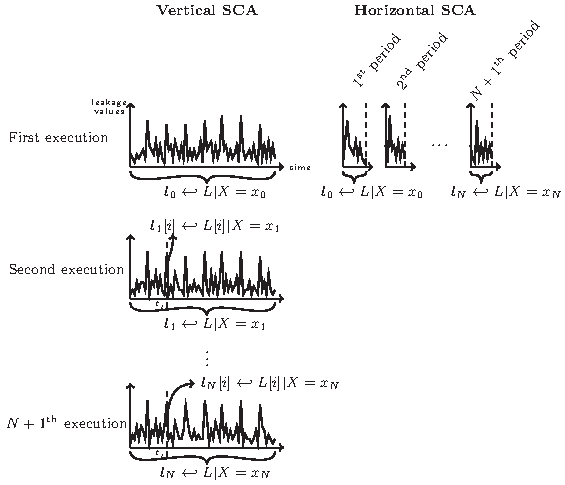
\includegraphics[scale=1.2]{vertical_and_horizontal_sca}
	\captionof{figure}{Visualization of Vertical and Horizontal SCAs (taken from \cite{bauer2013horizontal}).
	A realization of random variable $X$ is referred to as the corresponding lower-case letter $x$.
	A power trace $l_i$ for a given input $x_i$ is denoted as $l_i \hookleftarrow L \mid X = x_i $ (this notation sums up the event of a sample of observations of $L$ under the input $x_i$).
	}
	\label{fig: vertical_and_horizontal_sca}
\end{figure}
%
An OTA combines these two different approaches to SCAs. 
The attack works by acquiring one target trace from the device under attack.
Patterns of certain operations from this target trace are then compared to templates obtained from the attacker's device (which is a similar device running the same implementation).
Thus, an attacker requires only one \emph{target trace} from the \emph{target device}.
Only a single template trace per key-bit is necessary, which is obtained from the device of the attacker.
OTAs can be used to attack the secret scalar used in a scalar multiplication algorithm.
In practice, OTAs make the following assumptions about the attacker \cite{batina2014online, dugardin2016dismantling}:
%
\begin{itemize}
	\item The attacker knows the input point $\mathcal{P}$ that belongs to the trace of the target device;
	\item The attacker knows the implementation of the scalar multiplication algorithm and can compute intermediate values of this algorithm;
	\item The attacker can choose the input point on a device similar to the target device.
\end{itemize}
%
For the attack to work, at least one assignment in the exponentiation algorithm must be dependent on the value of particular scalar bit(s). 
However, there should not be any branches with key-dependent computations.
We now give a global overview of how an OTA works:
%
\begin{itemize}
	\item First, the attacker obtains a target trace with input point $\mathcal{P}$ from the target device;
	\item The attacker now obtains the template traces with input points $[m]P$ for $m \in \mathbb{Z}$.
	 This is done for multiples of the point $\mathcal{P}$, for example $2\mathcal{P}$ or $3\mathcal{P}$;
	 \item The attacker now compares the correlations between the target trace and each pair of template traces.
	 The one with the highest correlation is the one most likely to be correct.
\end{itemize}
%

\subsection{Creating the templates}
In \cite{batina2014online}, several examples are shown on how an OTA works for different scalar multiplication algorithms.
Consider the left-to-right double-and-add always algorithm shown in \Cref{Left-to-right double-and-add-always}.
%
\begin{algorithm}
	\algorithmicrequire $\bm{\mathcal{P}}$, $k = (1, k_{x-2}, \ldots, k_0)_2$. \\
	\algorithmicensure $\bm{Q} = k \cdot \bm{\mathcal{P}}$.
	%	
	\begin{algorithmic}[1]
		\State $\bm{R}_0 \gets \bm{\mathcal{P}}$ 
		\For{$i = x - 2$ \textbf{to} $0$}
			\State $\bm{R}_0 \gets 2 \bm{R}_0$
			\State $\bm{R}_1 \gets \bm{R}_0 + \bm{\mathcal{P}}$
			\State $\bm{R}_0 \gets \bm{R}_{k_i}$ \Comment{Depending on the bit value of $k_i$, $\bm{R}_0$ either takes the value $\bm{R}_0$ or $\bm{R}_1$}
		\EndFor
		\State \textbf{Return} $\bm{R}_0$
	\end{algorithmic}
	%
	\captionof{algorithm}{Left-to-right double-and-add-always algorithm \cite{batina2014online}.}
	\label{Left-to-right double-and-add-always}
\end{algorithm}
%
The algorithm assumes that the most-significant bit of the scalar $k$ is 1 (i.e. $k_\text{MSB} = 1$).
We now describe how an OTA can be applied in the case of \Cref{Left-to-right double-and-add-always}.
It is assumed that the first bit of the scalar is $1$.
However, if we take a look at the `for loop' in \Cref{Left-to-right double-and-add-always}, we see that this bit is not used.
Therefore, we assume that the first iteration of this algorithm (which involves a point doubling and addition) is done with the neutral element of the curve.
Thus, execution of the first iteration will yield the point $\mathcal{P}$.
If we now consider the second iteration (the operations that correspond to $k_\text{MSB} - 1$), we can verify that the expected outputs of this iteration are either $2 \mathcal{P}$ or $3 \mathcal{P}$ (depending on the value of $k_{\text{MSB} - 1}$). 
We now know that in the next iteration (i.e. the operations belonging to key-bit $k_{\text{MSB} - 2}$), a doubling of either $2 \mathcal{P}$ or $3 \mathcal{P}$ will be performed.
On our copy of the same device, we can now execute the algorithm with input point $2 \mathcal{P}$ or $3 \mathcal{P}$. This gives us a trace of the corresponding doubling operations.
Thus we can match the trace of the doubling operation in the ${(i + 1)}^\mathrm{th}$ iteration of the target trace with the appropriate template trace to attack the key bit used in the $i^\mathrm{th}$ iteration:
%
\begin{itemize}
	\item  If $k_{\text{MSB} - 1} = 0$, then the output of the second iteration is $2 \mathcal{P}$. The template trace for $2\mathcal{P}$ (obtained from the iteration involving $k_{\text{MSB} - 2}$) will now give a higher correlation with the target trace than the template trace for $3\mathcal{P}$.
	
	\item If $k_{\text{MSB} - 1} = 1$, then the output of the second iteration is $3 \mathcal{P}$. The template trace for $3\mathcal{P}$ (obtained from the iteration involving $k_{\text{MSB} - 2}$) will now give a higher correlation with the target trace than the template trace for $2\mathcal{P}$.
\end{itemize}
%
In this way, we can iteratively attack and retrieve all of the key bits used.
Note that when we calculate the correlation of the template trace with the target trace, we compare them only at the \emph{suitable} parts of the traces. 
These are the places at which the key-bit related assignments take place.
To determine the most likely key-bit, we compute the correlations with the target trace and the template traces, which in the second iteration would be $2\mathcal{P}$ and $3\mathcal{P}$. 
We consider the template trace that gives the highest correlation value as the one with the right key guess.
We repeat this procedure to find the key-bit for $k_{\text{MSB} - 2}$: we correlate the templates for $4\mathcal{P}$ and $5\mathcal{P}$ with the target trace if we guessed that $k_\text{MSB} - 1 = 0$.
Otherwise, we would correlate using the templates $6\mathcal{P}$ and $7\mathcal{P}$.
Again, the template that gives the highest correlation with the target trace is the most likely one to be correct.
An example of attacking the first two bits of a secret scalar $k$ with respect to \Cref{Left-to-right double-and-add-always} can be seen in \Cref{table: OTA example visualization}.
%
\begin{table}
	\centering
	%
	% Iteration 2 example
	%
	\subfloat[Attacking the second-most significant key bit $K_{\text{MSB} - 1}$. $\operatorname{D}$ and $\operatorname{A}$ stand for the doubling and addition operation respectively as performed in \Cref{Left-to-right double-and-add-always}. Depending on the correlation of the output of the operations performed using the key-bit $K_{\text{MSB} - 1}$ and the corresponding template traces (in this case the template trace $\operatorname{D}(2 \mathcal{P})$), we determine the most likely value for $K_{\text{MSB} - 1}$. In this iteration, we assume that the template for $\operatorname{D}(2 \mathcal{P})$ gives the highest correlation with the target trace.]{
	%
	\begin{tabular}{*7c}
		\toprule
		& \multicolumn{2}{c}{$K_{\text{MSB}} = 1$}  & \multicolumn{2}{c}{$K_{\text{MSB} - 1} \in \{\textcolor{red}{0}, \textcolor{blue}{1}\}$}  & \multicolumn{2}{c}{$K_{\text{MSB} - 2}$} \\
		\midrule
		\textbf{Target Trace} & $\operatorname{D}(\mathcal{O})$ & $\operatorname{A}(\mathcal{O}, \mathcal{P})$ & $\operatorname{D}(\mathcal{P})$ & $\operatorname{A}(2\mathcal{P}, \mathcal{P})$ & $\textcolor{red}{\operatorname{D}(2\mathcal{P})}$ \emph{or} $\textcolor{blue}{\operatorname{D}(3\mathcal{P})} $ & \\
		%
		\multicolumn{7}{c}{} \\
		%
		\textbf{Template Trace of $2 \mathcal{P}$}  & $\operatorname{D}(\mathcal{O})$ & $\operatorname{A}(\mathcal{O}, 2\mathcal{P})$ & \cellcolor{red!20} $\operatorname{D}(2\mathcal{P})$ & $\operatorname{A}(4\mathcal{P}, 2\mathcal{P})$ &  &  \\
		\bottomrule
	\end{tabular}
	%
	\label{table: OTA template matching iteration 2}
	}
	\vfill
	%
	% Iteration 3 example
	%
	\subfloat[Attacking the third-most significant key bit $K_{\text{MSB} - 2}$. 
	Depending on the correlation of the output of the operations performed using the key-bit $K_{\text{MSB} - 2}$ and the corresponding template traces (in this case the template trace $\operatorname{D}(4 \mathcal{P})$), we determine the most likely value for $K_{\text{MSB} - 2}$.]{
		% TODO manually scaled the textwidth, otherwise tablew would still be to wide
		\begin{adjustbox}{max width=.98\textwidth}
			%
			\begin{tabular}{*9c}
				\toprule
				& \multicolumn{2}{c}{$K_{\text{MSB}} = 1$}  & \multicolumn{2}{c}{$K_{\text{MSB} - 1} = 0$}  & \multicolumn{2}{c}{$K_{\text{MSB} - 2} \in \{\textcolor{red}{0}, \textcolor{blue}{1}\}$} & \multicolumn{2}{c}{$K_{\text{MSB} - 3}$} \\
				\midrule
				\textbf{Target Trace} & $\operatorname{D}(\mathcal{O})$ & $\operatorname{A}(\mathcal{O}, \mathcal{P})$ & $\operatorname{D}(\mathcal{P})$ & $\operatorname{A}(2\mathcal{P}, \mathcal{P})$ &
				$\operatorname{D}(2\mathcal{P})$ & $\operatorname{A}(4\mathcal{P}, \mathcal{P})$ & $\textcolor{red}{\operatorname{D}(4\mathcal{P})}$ \emph{or} $\textcolor{blue}{\operatorname{D}(5\mathcal{P})} $ & \\
				%
				\multicolumn{9}{c}{} \\
				%
				\textbf{Template Trace of $4 \mathcal{P}$}  & $\operatorname{D}(\mathcal{O})$ & $\operatorname{A}(\mathcal{O}, 4\mathcal{P})$ & \cellcolor{red!20} $\operatorname{D}(4\mathcal{P})$ & $\operatorname{A}(8\mathcal{P}, 4\mathcal{P})$ &  & & & \\
				\bottomrule
			\end{tabular}
		%
		\end{adjustbox}
		\label{table: OTA template matching iteration 3}
	}
	%
	\captionof{figure}{Visualization of the first two iterations of the OTA applied to \Cref{Left-to-right double-and-add-always} (tables based on examples shown in \cite{dugardin2016dismantling}).}
	\label{table: OTA example visualization}
\end{table}
%

\subsection{Matching the templates}
As mentioned previously, template matching is only performed with parts of the power trace at which the key-bit related assignments take place.
To calculate the correlation between a template and target trace such that we can distinguish the right hypothesis on the current bit under attack, we can make use of the Pearson correlation coefficient. 
The Pearson correlation coefficient is defined as follows:
%
\begin{equation*}
\rho(X, Y) = \frac{\operatorname{cov}(X, Y)}{\sigma_X \sigma_Y}
\end{equation*}
%
where $\operatorname{cov}$ is the covariance, $\sigma_X$ is the standard deviation of $X$ and $\sigma_Y$ is the standard deviation of $Y$.
$X$ and $Y$ would in this case be the template and target trace (in any order).